\PassOptionsToPackage{unicode}{hyperref}
\PassOptionsToPackage{naturalnames}{hyperref}

\documentclass[xcolor=dvipsnames, aspectratio=149, 12pt]{beamer}


\usepackage{etex}
%\usetheme{Darmstadt}
\usetheme{Madrid}
%\usecolortheme[named=NavyBlue]{structure}
\usecolortheme{whale}

%\usetheme{Frankfurt}  %\usecolortheme{default}

%\useoutertheme{infolines}

\mode<presentation>

\setbeamersize{text margin left=5mm}
\setbeamersize{text margin right=5mm}
\setbeamertemplate{footline}[page number]{}
\setbeamertemplate{blocks}[rounded][shadow=false]
\setbeamertemplate{title page}[default][colsep=-4bp,rounded=true]
\beamertemplatenavigationsymbolsempty
    %\setbeamertemplate{footline}{%
     % \raisebox{5pt}{\makebox[\paperwidth]{\hfill\makebox[10pt]{\scriptsize\insertframenumber}}}}
      
\addtobeamertemplate{block begin}{\setlength{\textwidth}{0.99\textwidth}}{}
\addtobeamertemplate{block begin}{\setlength\abovedisplayskip{0pt}}
%\addtobeamertemplate{block begin}{\vspace{-25pt}}{}


\usepackage{ucs}
\usepackage[utf8x]{inputenc}
\usepackage[greek,english]{babel}
\newcommand{\en}{\selectlanguage{english}}
\newcommand{\el}{\selectlanguage{greek}}
\usepackage[T1]{fontenc}
\usepackage{lmodern}

\usepackage[absolute,overlay]{textpos}

\newcommand{\sq}{\selectlanguage{english}\color{red!70!blue}\bf}
\newcommand{\bb}{\selectlanguage{greek}\color{blue!50!black}\bf}
\newcommand{\ra}{\selectlanguage{english}\color{blue!90!red}\em\large}
\newcommand{\enb}{\selectlanguage{english}\color{blue}}
\newcommand{\ex}[1]{\begin{math}\partial{#1}\end{math}}

\newcommand{\cgg}{\selectlanguage{english}\color{green!60!black}\bf}
\newcommand{\cmm}{\selectlanguage{english}\color{red!50!blue}\bf}

\newcommand{\cee}{\selectlanguage{greek}\color{red!90!blue}\bf\large}
\newcommand{\bbl}{\color{blue!90!black}\bf}
\newcommand{\crr}{\color{red!90!blue}\bf}
\newcommand{\cbb}{\color{blue!90!black}\bf}

\colorlet{colBC}{Apricot!50}

%\usepackage{enumitem}
\usepackage{booktabs}
\usepackage{hyperref}
\usepackage{listings}
\usepackage{fancyvrb}
\usepackage{listings}
\usepackage{amsmath}
\usepackage{amssymb}
\usepackage{mathtools}
\usepackage{mathrsfs}
\usepackage{colortbl}
\usepackage{graphicx}
\usepackage{chngcntr}
%\usepackage{subfig}
%\usepackage{subcaption}}
\usepackage{pgf, tikz}
\usepackage{pgfplots} %\pgfplotsset{compat=newest}
\usepackage{pgfplotstable}
\usepackage{comment}
\usepackage[normalem]{ulem}

\usepackage[tikz]{bclogo}
\usetikzlibrary{matrix}
\usetikzlibrary{arrows,automata,shapes,calc,positioning,fit}
\usetikzlibrary{backgrounds,shadows,trees}


\usetikzlibrary{calc}
%\usepackage{booktabs}
\usepackage{attachfile}

\definecolor{blue10}{RGB}{135, 204, 255}
\definecolor{blue90}{RGB}{0, 0, 204}


\DefineVerbatimEnvironment{codeE}{Verbatim}
{
  frame            = leftline,
  samepage         = true,
  commandchars     = &\{\}, 
  rulecolor=\color{black!50!white}, framerule=3px,
  baselinestretch  = 1,
  fontsize         = \small
}

\DefineVerbatimEnvironment{codeR}{Verbatim}
{
  frame            = leftline,
  samepage         = true,
  numbers          = left,
  numbersep        = 6pt,
  commandchars     = &\{\}, 
  rulecolor=\color{red!90!black}, framerule=3px,
  baselinestretch  = 1,
  fontsize         = \small
}

\DefineVerbatimEnvironment{codeM}{Verbatim}
{
  frame=leftline,  framerule=2px,  rulecolor=\color{blue},
  samepage=true, numbers=left,   numbersep=6pt,
  commandchars=&\{\}, baselinestretch=1, fontsize=\small
}

\DefineVerbatimEnvironment{codeO}{Verbatim}
{
  frame=leftline,  framerule=2px,  rulecolor=\color{blue},
  samepage=true, numbers=left,   numbersep=6pt,
  commandchars=&\{\}, baselinestretch=1, fontsize=\small
}

\DefineVerbatimEnvironment{SQL}{Verbatim}
{
  frame=leftline,  framerule=2px,  rulecolor=\color{blue},
  samepage=true, numbers=left,   numbersep=6pt,
  commandchars=&\{\}, baselinestretch=1, fontsize=\small
}

\DefineVerbatimEnvironment{codeC}{Verbatim}
{
  frame=leftline,  framerule=2px,  rulecolor=\color{blue},
  samepage=true, numbers=left,   numbersep=6pt,
  commandchars=&\{\}, baselinestretch=1, fontsize=\small
}


\newcommand{\code}[1]{\en \textsl{#1}}{\el}
\newcommand{\ojoinaux}{\setbox0=\hbox{$\bowtie$}%
  \rule[-.02ex]{.25em}{.4pt}\llap{\rule[\ht0]{.25em}{.4pt}}}
\newcommand{\ojoin}{\mathbin{\ojoinaux\mkern-5.6mu\bowtie\mkern-5.7mu\ojoinaux}}
\newcommand{\lojoin}{\mathbin{\ojoinaux\mkern-5.6mu\bowtie}}
\newcommand{\rojoin}{\mathbin{\bowtie\mkern-5.7mu\ojoinaux}}

\newcommand{\stirlingtwo}[2]{\genfrac{\lbrace}{\rbrace}{0pt}{}{#1}{#2}}

\logo{\includegraphics[width=2.5cm,height=2.5cm,keepaspectratio]{../common/SQL2.jpg}}

\AtBeginSection[]
{ \el
  \begin{frame}<beamer>
    \frametitle{Περιεχόμενα}
    \begin{minipage}{\wE}
      \tableofcontents[currentsection]
    \end{minipage} 
  \end{frame}
}

\AtBeginSubsection[]
{
  \begin{frame}<beamer>
    \frametitle{Περιεχόμενα}
    \begin{minipage}{\wE}
      \tableofcontents[currentsubsection]
    \end{minipage}   
  \end{frame}
}


\newcommand{\wE}{0.88\textwidth}
\newcommand{\wN}{0.92\textwidth}



\newcommand{\men}[1] {\selectlanguage{english}#1\selectlanguage{greek}}
\newcommand{\mene}[1] {\selectlanguage{english}\emph{#1}\selectlanguage{greek}}
\newcommand{\mgr}[1] {\selectlanguage{greek}#1\selectlanguage{english}}
\newcommand{\mgre}[1] {\selectlanguage{greek}\emph{#1}\selectlanguage{english}}


% η \tsql τυπώνει SQL
\newcommand{\tsql}{\selectlanguage{english}SQL\selectlanguage{greek}}
\newcommand{\tasql}{\selectlanguage{english}ANSI-SQL\selectlanguage{greek}}
\newcommand{\tddl}{\selectlanguage{english}DDL\selectlanguage{greek}}
\newcommand{\tdml}{\selectlanguage{english}DML\selectlanguage{greek}}

\newcommand{\tselect}{\selectlanguage{english}SELECT\selectlanguage{greek}}
\newcommand{\tselectd}{\selectlanguage{english} SELECT$\ldots$ \selectlanguage{greek}}
\newcommand{\tfrom}{\selectlanguage{english}FROM\selectlanguage{greek}}
\newcommand{\tfromd}{\selectlanguage{english} FROM$\ldots$ \selectlanguage{greek}}
\newcommand{\twhere}{\selectlanguage{english}WHERE\selectlanguage{greek}}
\newcommand{\twhered}{\selectlanguage{english} WHERE $\ldots$\selectlanguage{greek}}
\newcommand{\torderby}{\selectlanguage{english}ORDER BY\selectlanguage{greek}}
\newcommand{\tgroupby}{\selectlanguage{english}GROUP BY\selectlanguage{greek}}
\newcommand{\thaving}{\selectlanguage{english}HAVING\selectlanguage{greek}}
\newcommand{\trollup}{\selectlanguage{english}ROLLUP\selectlanguage{greek}}
\newcommand{\tnull}{\selectlanguage{english}NULL\selectlanguage{greek}}
\newcommand{\tunk}{\selectlanguage{english}UNK\selectlanguage{greek}}
\newcommand{\tnotnull}{\selectlanguage{english}NOT NULL\selectlanguage{greek}}
\newcommand{\ttrue}{\selectlanguage{english}TRUE\selectlanguage{greek}}
\newcommand{\tfalse}{\selectlanguage{english}FALSE\selectlanguage{greek}}
\newcommand{\tlike}{\selectlanguage{english}LIKE\selectlanguage{greek}}
\newcommand{\tand}{\selectlanguage{english}AND\selectlanguage{greek}}
\newcommand{\tor}{\selectlanguage{english}OR\selectlanguage{greek}}
\newcommand{\tnot}{\selectlanguage{english}NOT\selectlanguage{greek}}
\newcommand{\tdistinct}{\selectlanguage{english}DISTINCT\selectlanguage{greek}}
\newcommand{\tavg}{\selectlanguage{english}AVG()\selectlanguage{greek}}
\newcommand{\tsum}{\selectlanguage{english}SUM()\selectlanguage{greek}}
\newcommand{\tmin}{\selectlanguage{english}MIN()\selectlanguage{greek}}
\newcommand{\tmax}{\selectlanguage{english}MAX()\selectlanguage{greek}}
\newcommand{\tcount}{\selectlanguage{english}COUNT()\selectlanguage{greek}}
\newcommand{\tcounta}{\selectlanguage{english}COUNT(*)\selectlanguage{greek}}
\newcommand{\tall}{\selectlanguage{english}ALL\selectlanguage{greek}}
\newcommand{\tany}{\selectlanguage{english}ANY\selectlanguage{greek}}
\newcommand{\texists}{\selectlanguage{english}EXISTS\selectlanguage{greek}}
\newcommand{\tdefault}{\selectlanguage{english}DEFAULT\selectlanguage{greek}}
\newcommand{\tconstraint}{\selectlanguage{english}CONSTRAINT\selectlanguage{greek}}
\newcommand{\tondelcas}{\selectlanguage{english}ON DELETE CASCADE\selectlanguage{greek}}
\newcommand{\tonupcas}{\selectlanguage{english}ON UPDATE CASCADE\selectlanguage{greek}}

\newcommand{\tjoin}{\selectlanguage{english}JOIN\selectlanguage{greek}}

\newcommand{\tinsert}{\selectlanguage{english}INSERT\selectlanguage{greek}}
\newcommand{\tdelete}{\selectlanguage{english}DELETE\selectlanguage{greek}}
\newcommand{\tupdate}{\selectlanguage{english}UPDATE\selectlanguage{greek}}

\newcommand{\tcreatedb}{\selectlanguage{english}CREATE DATABASE\selectlanguage{greek}}
\newcommand{\tcreatetab}{\selectlanguage{english}CREATE TABLE\selectlanguage{greek}}
\newcommand{\taltertab}{\selectlanguage{english}ALTER TABLE\selectlanguage{greek}}
\newcommand{\tprikey}{\selectlanguage{english}PRIMARY KEY\selectlanguage{greek}}
\newcommand{\tforkey}{\selectlanguage{english}FOREIGN KEY\selectlanguage{greek}}
\newcommand{\tdropt}{\selectlanguage{english}DROP TABLE\selectlanguage{greek}}
\newcommand{\tdropv}{\selectlanguage{english}DROP VIEW\selectlanguage{greek}}

\newcommand{\tgrant}{\selectlanguage{english}GRANT\selectlanguage{greek}}
\newcommand{\trevoke}{\selectlanguage{english}REVOKE\selectlanguage{greek}}

\newcommand{\tmysql}{\selectlanguage{english}MySQL\selectlanguage{greek}}
\newcommand{\taccess}{\selectlanguage{english}MS ACCESS\selectlanguage{greek}}
\newcommand{\toracle}{\selectlanguage{english}ORACLE\selectlanguage{greek}}
\newcommand{\tsybase}{\selectlanguage{english}Sybase\selectlanguage{greek}}
\newcommand{\tapache}{\selectlanguage{english}Apache\selectlanguage{greek}}
\newcommand{\tphp}{\selectlanguage{english}PHP\selectlanguage{greek}}


\newcommand{\tunion}{\selectlanguage{english}UNION\selectlanguage{greek}}
\newcommand{\tuniona}{\selectlanguage{english}UNION ALL\selectlanguage{greek}}
\newcommand{\tuniond}{\selectlanguage{english}UNION DISTINCT\selectlanguage{greek}}
\newcommand{\tintersect}{\selectlanguage{english}INTERSECT\selectlanguage{greek}}

\newcommand{\tcom}{$=,<>,<,<=,>,>=$}

\newcommand{\kb}{\selectlanguage{english}KBytes\selectlanguage{greek}}
\newcommand{\mb}{\selectlanguage{english}MBytes\selectlanguage{greek}}
\newcommand{\gb}{\selectlanguage{english}GBytes\selectlanguage{greek}}

\newcommand{\tdbms}{Σύστημα Διαχείρισης Βάσεων Δεδομένων}
\newcommand{\trdbms}{Σχεσιακό Σύστημα Διαχείρισης Βάσεων Δεδομένων}
\newcommand{\tdbmsg}{Συστήματος Διαχείρισης Βάσεων Δεδομένων}
\newcommand{\tdbmss}{Συστήματα Διαχείρισης Βάσεων Δεδομένων}
\newcommand{\trdbmss}{Σχεσιακά Συστήματα Διαχείρισης Βάσεων Δεδομένων}
\newcommand{\terd}{Διάγραμμα Οντοτήτων/Συσχετίσεων}
\newcommand{\terdb}{Διαγράμματος Οντοτήτων/Συσχετίσεων}
\newcommand{\ter}{Οντοτήτων/Συσχετίσεων}

\newcommand{\tcompany}{\selectlanguage{english}{\bf COMPANY}\selectlanguage{greek}}
\newcommand{\temployees}{\selectlanguage{english}\emph{employees}\selectlanguage{greek}}
\newcommand{\tdepartments}{\selectlanguage{english}\emph{departments}\selectlanguage{greek}}
\newcommand{\tprojects}{\selectlanguage{english}\emph{projects}\selectlanguage{greek}}
\newcommand{\tworkson}{\selectlanguage{english}\emph{workson}\selectlanguage{greek}}

\newcommand{\tdepid}{\selectlanguage{english}\emph{depid}\selectlanguage{greek}}
\newcommand{\tdepname}{\selectlanguage{english}\emph{depname}\selectlanguage{greek}}
\newcommand{\tmanager}{\selectlanguage{english}\emph{manager}\selectlanguage{greek}}

\newcommand{\tempid}{\selectlanguage{english}\emph{empid}\selectlanguage{greek}}
\newcommand{\tfirstname}{\selectlanguage{english}\emph{firstname}\selectlanguage{greek}}
\newcommand{\tlastname}{\selectlanguage{english}\emph{lastname}\selectlanguage{greek}}
\newcommand{\tsalary}{\selectlanguage{english}\emph{salary}\selectlanguage{greek}}
%\newcommand{\thiredate}{\selectlanguage{english}\emph{hiredate}}\selectlanguage{greek}}

\newcommand{\tproid}{\selectlanguage{english}\emph{proid}\selectlanguage{greek}}
\newcommand{\ttitle}{\selectlanguage{english}\emph{title}\selectlanguage{greek}}
\newcommand{\tbudget}{\selectlanguage{english}\emph{budget}\selectlanguage{greek}}


\newcommand{\attention}{\marginpar{\hfill\fbox{\Large{!}}}}
\newcommand{\tthink}{\selectlanguage{english} \textbf{\emph{Think in SQL and have a great fun!}} \selectlanguage{greek}}


\newcommand{\logomysql}{\marginpar{\hfill{\includegraphics[scale=0.7]{mysql.jpg}}}}
\newcommand{\logoaccess}{\marginpar{\hfill{\includegraphics[scale=0.7]{access.jpg}}}}
\newcommand{\logooracle}{\marginpar{\hfill{\includegraphics[scale=0.8]{oracle.jpg}}}}

\newcommand{\igok}    {\includegraphics[scale=1.0] {pics/OK.png}}
\newcommand{\igcancel}{\includegraphics[scale=1.0] {pics/cancel.png}}
\newcommand{\igadd}   {\includegraphics[scale=1.0] {pics/add.png}}
\newcommand{\igclose} {\includegraphics[scale=1.0] {pics/close.png}}

\newcommand{\calg} {\mathscr{G}}

\newcommand{\tsummary} {\clearpage  \section{\el Περίληψη κεφαλαίου}} 
\newcommand{\tautoeval} {\clearpage  \section{\el Ερωτήσεις αυτοαξιολόγησης}} 
\newcommand{\trepeatexer} {\clearpage  \section{\el Ασκήσεις επανάληψης}} 

\newcommand{\nf} {κανονική μορφή} 
\newcommand{\anf} {1\textsuperscript{η} κανονική μορφή} 
\newcommand{\bnf} {2\textsuperscript{η} κανονική μορφή} 
\newcommand{\cnf} {3\textsuperscript{η} κανονική μορφή} 
\newcommand{\bcnf} {\men{Boyce--Codd} κανονική μορφή} 
\newcommand{\dnf} {4\textsuperscript{η} κανονική μορφή}
\newcommand{\enf} {5\textsuperscript{η} κανονική μορφή}
\newcommand{\fnf} {6\textsuperscript{η} κανονική μορφή}   


\newcommand{\maxcard}{\mathop{\mathrm{maxcard}}}
\newcommand{\mincard}{\mathop{\mathrm{mincard}}}


\begin{document}
\el
\author[]{Αθανάσιος Σταυρακούδης}
\title[]{Το σχεσιακό μοντέλο δεδομένων}
\date[]{Άνοιξη 2016}
\institute{\en \texttt{http://stavrakoudis.econ.uoi.gr}}

{
\setbeamertemplate{footline}{}
\begin{frame}%[t, fragile, shrink]
  \titlepage
\end{frame}
}
\addtocounter{framenumber}{-1}


%\section[\textlatin{Codd Rules}]{\textgreek{Οι 12 κανόνες του} \textlatin{E.F. Codd}}

\section[\textlatin{Codd Rules}]{\textgreek{Οι 12 κανόνες του} \textlatin{Codd}}


\begin{frame}[t,fragile]
\frametitle{\en Edgar F. Codd}
\begin{columns}[T]
  \begin{column}{0.65\textwidth}
    \begin{itemize}
      \item Άγγλος επιστήμονας, 1923 -- 2003.
      \item Θεμελιωτής του σχεσιακού μοντέλου βάσεων δεδομένων.
      \item Πιλότος στο 2ο παγκόσμιο πόλεμο.
      \item Εργάστηκε πολλά χρόνια για την {\en IBM}.
      \item Περισσότερο γνωστός για την εργασία του 
           {\en\color{blue} "A Relational Model of Data for Large Shared Data Banks".\footnote{\url{http://dl.acm.org/citation.cfm?doid=362384.362685}}}
      \item Βραβείο {\sq Turing} το 1981.     
    \end{itemize}
  \end{column}
  \begin{column}{0.35\textwidth} \hspace*{-2cm}
    \includegraphics[scale=0.8]{Edgar_F_Codd.jpg}
  \end{column}
\end{columns}
\end{frame}



\begin{frame}[t,fragile]
\frametitle{Κανόνας $\# 1$ }
\begin{minipage}{\wE}
  \en
  \begin{bclogo} [couleur=colBC, logo=\bccrayon, arrondi=0.1, couleurBord=red!80!blue, barre=none] {The information Rule}
    \em
      All information in a relational database (including table and column names) is represented in only one way, namely as a value in a table.
  \end{bclogo}
  \el
  \begin{block}{\en The information rule}
     Όλα τα δεδομένα και οι πληροφορίες της βάσης αναπαριστώνται
     στο λογικό επίπεδο της βάσης δεδομένων μέσα σε πίνακες.
  \end{block}
\end{minipage}
\end{frame}



\begin{frame}[t,fragile]
\frametitle{Κανόνας $\# 2$ }
\begin{minipage}{\wE}
  \en
  \begin{bclogo} [couleur=colBC, logo=\bccrayon, arrondi=0.1, couleurBord=red!80!blue, barre=none] {The guaranteed access rule}
    \em
      All data must be accessible. 
      This rule is essentially a restatement of the fundamental requirement for primary keys. 
      It says that every individual scalar value in the database must be logically addressable 
      by specifying the name of the containing table, the name of the containing column 
      and the primary key value of the containing row.
  \end{bclogo}
  \el
  \begin{block}{\en The guaranteed access rule}
     Με βάση το λογικό επίπεδο της βάσης, όλα τα δεδομένα μπορούν
     να προσπελαστούν με βάση τον πίνακα στον οποίο έχουν καταχωρηθεί,
     με την τιμή του πρωτεύοντος κλειδιού, και το όνομα της στήλης του πίνακα.
  \end{block}
\end{minipage}
\end{frame}


\begin{frame}[t,fragile]
\frametitle{Κανόνας $\# 3$ }
\begin{minipage}{\wE}
  \en
  \begin{bclogo} [couleur=colBC, logo=\bccrayon, arrondi=0.1, couleurBord=red!80!blue, barre=none] {Systematic treatment of null values:}
    \em
      The DBMS must allow each field to remain null (or empty). Specifically, it must support a representation of "missing information and inapplicable information" that is systematic, distinct from all regular values (for example, "distinct from zero or any other number", in the case of numeric values), and independent of data type. 
      It is also implied that such representations must be manipulated by the DBMS in a systematic way.
  \end{bclogo}
  \el
  \begin{block}{}%{\en The guaranteed access rule}
     Οι τιμές {\sq \tnull} πρέπει να χρησιμοποιούνται ως ελλιπής πληροφορία,
        όχι ως μηδενικές αριθμητικές τιμές, κενά αλφαριθμητικά ή ο κενός
        χαρακτήρας (\men{space}).
  \end{block}
\end{minipage}
\end{frame}


\el
\section[\textgreek{Περιγραφή}] {\textgreek {Κεντρικές έννοιες του σχεσιακού μοντέλου} }

\subsection[\textgreek{Περί}]{\textgreek{Ορισμοί για τις σχέσεις}}

\begin{frame}[t, fragile, shrink]
\frametitle{Τι είναι σχέση?}
\begin{minipage}{\wE}
  \begin{tabular}{ c l c } \toprule
    {\bf Κωδικός} & {\bf Όνομα} & {\bf Εξάμηνο} \\ \midrule 
    504 & Βάσεις Δεδομένων & 5 \\ 
    404 & Μακροοικονομική Θεωρία ΙΙ & 4 \\  
    303 & Προγραμματισμός Υπολογιστών Ι & 3 \\   
    604 & Πληροφοριακά Συστήματα Διοίκησης & 6 \\  \bottomrule
  \end{tabular}
  \bigskip \par Η πιο απλή πρακτική αναπαράσταση μιας σχέσης, είναι ένας πίνακας
  δεδομένων δύο διαστάσεων.
  Το παραπάνω σχήμα  απεικονίζει ένα παράδειγμα μιας σχέσης: της σχέσης {\bb μάθημα} από
  το πρόγραμμα σπουδών ενός τμήματος πανεπιστημίου. 
\end{minipage}
\end{frame}


\begin{frame}[t, fragile, shrink]
\frametitle{Αντιστοιχία πίνακα με σχέση}
\begin{minipage}{\wE}
  \pause
  \begin{enumerate}[<+->] \itemsep 6pt
    \item Η αντιστοιχία είναι άτυπη, μια σχέση δεν είναι ακριβώς ένας πίνακας.
    \item Η σχέση έχει μια {\crr επικεφαλίδα}, την πρώτη
          γραμμή του πίνακα, που συνιστά το {\crr σχήμα της σχέσης}.
    \item Το σχήμα της σχέσης είναι ένα
          σύνολο από γνωρίσματα, πχ  \{Κωδικός, Όνομα, Εξάμηνο\}.
    \item Το σύνολο \{504, Βάσεις Δεδομένων, 5\} 
          είναι μια πλειάδα (ή συστοιχία) της σχέσης {\crr Μαθήματα}.
    \item Μια σχέση έχει ακριβώς ένα καθορισμένο σχήμα, 
          έχει όμως, ενδεχομένως, πολλές πλειάδες.
    \item Οι τιμές κάθε γνωρίσματος προέρχονται από το κάποιο {\crr πεδίο ορισμού}.
\end{enumerate}
\end{minipage}
\end{frame}


\begin{frame}[t, fragile, shrink]
\frametitle{Διευκρινίσεις για τις σχέσεις}
\begin{minipage}{\wE}
  \pause
  \begin{enumerate}[<+->] \itemsep 3pt
    \item Μια σχεσιακή βάση δεδομένων καταγράφει δεδομένα μέσα σε {\crr σχέσεις}, 
          και μόνο σε αυτές.
    \item Αντικείμενα και γεγονότα γίνονται αντιληπτά στη βάση δεδομένων,
          ως τιμές που αντιστοιχούν στα {\crr γνωρίσματα} μιας σχέσης.
    \item Η σχέση είναι ένα {\crr σύνολο από γνωρίσματα}, το καθένα με διαφορετικό όνομα,
          και κάποιο πεδίο ορισμού.
    \item Η πλειάδα είναι ένα {\crr σύνολο από τιμές} που προέρχονται από το πεδίο τιμών του κάθε γνωρίσματος.
    \item Μια σχέση έχει ένα καθορισμένο σύνολο γνωρισμάτων, 
          το οποίο γενικά μένει σταθερό ως προς το χρόνο χρήσης
          της βάσης δεδομένων.
    \item Το σύνολο αυτό λέγεται επικεφαλίδα της σχέσης, ή {\crr σχήμα της σχέσης}. 
  \end{enumerate}
\end{minipage}
\end{frame}


\begin{frame}[t, fragile, shrink]
\frametitle{Ενημέρωση σχέσεων}
\begin{minipage}{\wE}
  \pause
  \begin{enumerate}[<+->] \itemsep 6pt
    \item Με τον όρο {\crr ενημέρωση} της  βάσης δεδομένων εννοείται η ενημέρωση μιας
         (ή και περισσότερων) σχέσης (ή σχέσεων) της βάσης δεδομένων.
    \item Η ενημέρωση μιας σχέσης γίνεται με την έννοια της {\crr πλειάδας},
          ενός συνόλου τιμών που αντιστοιχούν στα γνωρίσματα της σχέσης.
    \item Η ενημέρωση γίνεται με τρεις πράξεις:
          \begin{itemize}
            \item Εισαγωγή πλειάδων
            \item Διαγραφή πλειάδων
            \item Τροποποίηση πλειάδων
          \end{itemize}
  \end{enumerate}
\end{minipage}
\end{frame}



\begin{frame}[t, fragile, shrink]
\frametitle{Ενημέρωση σχέσεων : Τροποποίηση}
  \vspace{-0.2cm}
  \begin{tabular}{ c p{7cm} c } \toprule
    {\bf Κωδικός} & {\bf Όνομα} & {\bf Εξάμηνο} \\ \midrule 
    504 & Βάσεις Δεδομένων & 5 \\ 
    404 & Μακροοικονομική Θεωρία ΙΙ & 4 \\  
    303 & \sout{Προγραμματισμός Υπολογιστών Ι}  \newline{} Εισαγωγή στον Προγραμματισμό & 3 \\   
    604 & Πληροφοριακά Συστήματα Διοίκησης & 6 \\  \bottomrule
  \end{tabular}
  \vspace{-0.5cm}
  \begin{minipage}{\wE}
    \begin{exampleblock}{Παράδειγμα} \small
      Αν το όνομα του μαθήματος {\cbb ((Προγραμματισμός Υπολογιστών Ι))} αλλάξει 
      σε {\crr ((Εισαγωγή στον Προγραμματισμό))}
      τότε αυτό που τροποποιήθηκε είναι η
      {\crr πλειάδα} με κωδικό 303. \\
      Άλλαξε δηλαδή τιμές κάποιο σύνολο καθώς η
      μεταβολή μιας τιμής μεταβάλει όλο το σύνολο τιμών, η {\crr ενημέρωση} των σχέσεων
      γίνεται {\crr κατά πλειάδες}.
    \end{exampleblock}
  \end{minipage}
\end{frame}



\begin{frame}[t, fragile, shrink]
\frametitle{Σχήμα σχέσης}
\begin{minipage}{\wE}
  \begin{block}{Σχήμα σχέσης}
    Σχήμα μιας σχέσης είναι το σύνολο των γνωρισμάτων της.
      \[ R (A_1, A_2, \ldots, A_n) \]
  \end{block}
  \begin{tabular}{ c l c } \toprule
    {\bf Κωδικός} & {\bf Όνομα} & {\bf Εξάμηνο} \\ \midrule 
    504 & Βάσεις Δεδομένων & 5 \\ 
    404 & Μακροοικονομική Θεωρία ΙΙ & 4 \\  
    303 & Προγραμματισμός Υπολογιστών Ι & 3 \\   
    604 & Πληροφοριακά Συστήματα Διοίκησης & 6 \\  \bottomrule
  \end{tabular}
  \begin{exampleblock}{}%{Παράδειγμα}
    Το σύνολο $\{ \text{Κωδικός}, \text{Όνομα}, \text{Εξάμηνο} \}$
    είναι το σχήμα της σχέσης Μαθήματα.
    \vspace{-4mm}
    {\bf\color{blue} \[ \text{Μαθήματα(\underline{Κωδικός}, Όνομα, Εξάμηνο)} \] }
  \end{exampleblock}
\end{minipage}   
\end{frame}


\begin{frame}[t, fragile, shrink]
\frametitle{Στιγμιότυπο σχέσης}
  \begin{block}{Στιγμιότυπο σχέσης}
    Στιγμιότυπο σχέσης που συμβολίζεται με $t[R]$ είναι το σύνολο όλων των πλειάδων μιας σχέσης
    μια συγκεκριμένη χρονική στιγμή.
 \end{block}
  \begin{tabular}{ c l c } \toprule
    {\bf Κωδικός} & {\bf Όνομα} & {\bf Εξάμηνο} \\ \midrule 
    504 & Βάσεις Δεδομένων & 5 \\ 
    404 & Μακροοικονομική Θεωρία ΙΙ & 4 \\  
    303 & Προγραμματισμός Υπολογιστών Ι & 3 \\   
    604 & Πληροφοριακά Συστήματα Διοίκησης & 6 \\  \bottomrule
  \end{tabular} 
\end{frame}


\begin{frame}[t, fragile, shrink]
\frametitle{Γνώρισμα σχέσης}
  \begin{block}{Γνώρισμα}
    Γνώρισμα της σχέσης (πεδίο ή στήλη ενός πίνακα) είναι μια ιδιότητα της σχέσης
    και έχει ένα μοναδικό όνομα μέσα στη σχέση.
  \end{block}
\begin{minipage}{0.94\textwidth}
  \begin{tabular}{ c l c } \toprule
    {\bf Κωδικός} & {\bf Όνομα} & {\bf Εξάμηνο} \\ \midrule 
    504 & Βάσεις Δεδομένων & 5 \\ 
    404 & Μακροοικονομική Θεωρία ΙΙ & 4 \\  
    303 & Προγραμματισμός Υπολογιστών Ι & 3 \\   
    604 & Πληροφοριακά Συστήματα Διοίκησης & 6 \\  \bottomrule
  \end{tabular}
  \begin{exampleblock}{Παράδειγμα}
    Ο {\bf Κωδικός}, το {\bf Όνομα} και το {\bf Εξάμηνο} του μαθήματος
    είναι γνωρίσματα της σχέσης.
  \end{exampleblock}  
\end{minipage}  
\end{frame}


\begin{frame}[t, fragile]
\frametitle{Πεδίο ορισμού γνωρίσματος σχέσης}
\begin{minipage}{\wE}
  \begin{block}{Πεδίο ορισμού}
    Πεδίο ορισμού $dom(A_i)$ ενός γνωρίσματος $(A_i)$ είναι όλες οι επιτρεπτές τιμές
    του γνωρίσματος $A_i$.
  \end{block}
  \begin{tabular}{ c l c } \toprule
    {\bf Κωδικός} & {\bf Όνομα} & {\bf Εξάμηνο} \\ \midrule 
    504 & Βάσεις Δεδομένων & 5 \\ 
    404 & Μακροοικονομική Θεωρία ΙΙ & 4 \\  
    303 & Προγραμματισμός Υπολογιστών Ι & 3 \\   
    604 & Πληροφοριακά Συστήματα Διοίκησης & 6 \\  \bottomrule
  \end{tabular}
  \begin{exampleblock}{Παράδειγμα}
    Πεδίο ορισμού του γνωρίσματος {\bf Εξάμηνο} είναι το σύνολο των ακεραίων αριθμών
    $\{1,2,3,4,5,6,7,8\}$.
  \end{exampleblock}
\end{minipage}  
\end{frame}


\begin{frame}[t, fragile, shrink]
\frametitle{Συστοιχία ή πλειάδα}
\begin{minipage}{\wE}
  \begin{block}{Συστοιχία ή πλειάδα}
    {\cee Συστοιχία ή πλειάδα} είναι μια διατεταγμένη λίστα από τιμές  $t=\,\,\,<v_1,v_2,\ldots,v_n>$,
    που κάθε μία ανήκει στο πεδίο
    ορισμού $dom(A_i)$ του αντίστοιχου γνωρίσματος $A_i$.
  \end{block}
  \begin{tabular}{ c l c } \toprule
    {\bf Κωδικός} & {\bf Όνομα} & {\bf Εξάμηνο} \\ \midrule 
    504 & Βάσεις Δεδομένων & 5 \\   \bottomrule
  \end{tabular}
  \bigskip \par Η διατεταγμένη λίστα τιμών 
    \[ t =\,\,\, <504, {\el\text{Βάσεις Δεδομένων}}, 5> \] 
     είναι μια συστοιχία ή πλειάδα της σχέσης.
\end{minipage}
\end{frame}


\begin{frame}[t, fragile, shrink]
\frametitle{Ορισμός σχέσης}
\begin{minipage}{\wE}
  \begin{block}{Σχέση}
    Είναι ο συνδυασμός του σχήματος $R$ και του στιγμιότυπου $r$ της σχέσης. 
  \end{block}
  \pause
  \begin{exampleblock}{Σχέση}
    Γράφουμε $r(R)$ και διαβάζουμε:\\
    \begin{itemize}
      \item Μια σχέση $r$ πάνω στο σχήμα $R$.
      \item Στιγμυότυπο $r$ του (σχεσιακού) σχήματος $R$.
    \end{itemize}

  \end{exampleblock}
\end{minipage}
\end{frame}


\begin{frame}[t, fragile, shrink]
\frametitle{Βαθμός σχέσης}
\begin{minipage}{\wE}
  \begin{block}{Βαθμός σχέσης}
    Βαθμός μιας σχέσης $r(R)$ είναι το πλήθος των γνωρισμάτων της σχέσης.
  \end{block}
  \pause
  \begin{exampleblock}{Μία σχέση με βαθμό 3}
    \begin{tabular}{ c l c } \toprule
        {\bf Κωδικός} & {\bf Όνομα} & {\bf Εξάμηνο} \\ \midrule
        504 & Βάσεις Δεδομένων & 5 \\
        404 & Μακροοικονομική Θεωρία ΙΙ & 4 \\
        303 & Προγραμματισμός Υπολογιστών Ι & 3 \\
        604 & Πληροφοριακά Συστήματα Διοίκησης & 6 \\ \bottomrule
    \end{tabular}    
  \end{exampleblock}
\end{minipage}  
\end{frame}


\begin{frame}[t, fragile, shrink]
\frametitle{Πληθικότητα σχέσης}
\begin{minipage}{\wE}
  \begin{block}{Πληθικότητα σχέσης}
    Πληθικότητα μιας σχέσης $r(R)$ είναι το πλήθος των πλειάδων της σχέσης.
  \end{block}
  \pause
  \begin{exampleblock}{Μία σχέση με πληθικότητα 4}
    \begin{tabular}{ c l c } \toprule
        {\bf Κωδικός} & {\bf Όνομα} & {\bf Εξάμηνο} \\ \midrule
        504 & Βάσεις Δεδομένων & 5 \\
        404 & Μακροοικονομική Θεωρία ΙΙ & 4 \\
        303 & Προγραμματισμός Υπολογιστών Ι & 3 \\
        604 & Πληροφοριακά Συστήματα Διοίκησης & 6 \\ \bottomrule
    \end{tabular}    
  \end{exampleblock} 
\end{minipage}  
\end{frame}


\begin{frame}[t, fragile, shrink]
\frametitle{Σχήμα της βάσης} 
\begin{minipage}{\wE}
  \begin{block}{Σχήμα της βάσης δεδομένων}
    Είναι το σύνολο των σχέσεων που αποτελούν τη βάση δεδομένων.
  \end{block}
    \pause
    \begin{exampleblock}{Παράδειγμα}
      \par Μαθήματα(Κωδικός, Όνομα, Εξάμηνο) \\ 
      \par \bigskip Αίθουσες(Κωδικός, Όνομα, Χωρητικότητα) \\
      \par \bigskip Πρόγραμμα(ΚωδΜαθ, ΚωδΑιθ, Ημέρα, Ώρα) \\
  \end{exampleblock}
\end{minipage}
\end{frame}



\subsection[\textgreek{Ιδιότητες}]{\textgreek{Οι 4 βασικές ιδιότητες των σχέσεων}}


\begin{frame}[t, fragile, shrink]
\frametitle{Ιδιότητες των σχέσεων}
\begin{minipage}{\wE}
\pause
\begin{enumerate} [<+->] \itemsep 6pt
  \item {\cee Μοναδικότητα πλειάδων.} Σε μια σχέση, όλες οι πλειάδες (συστοιχίες) είναι μοναδικές.
        Δεν υπάρχουν επαναλαμβανόμενες πλειάδες.
  \item {\cee Διάταξη πλειάδων.} Δεν υπάρχει συγκεκριμένη διάταξη (ταξινόμηση) των πλειάδων σε μια σχέση.
  \item {\cee Διάταξη γνωρισμάτων.} Δεν υπάρχει επίσης, διάταξη των γνωρισμάτων μιας σχέσης.
        Τα γνωρίσματα δεν είναι διατεταγμένα πχ, από τα αριστερά προς τα δεξιά.
  \item {\cee Ατομικότητα.} Κάθε γνώρισμα έχει μια μόνο τιμή σε μια συγκεκριμένη πλειάδα.
\end{enumerate}
\end{minipage}
\end{frame}


\begin{frame}[t, fragile, shrink]
\frametitle{Μοναδικότητα}
\begin{tabular}{ c l l l } \hline 
	{\bf ΑΦΜ} & {\bf Επώνυμο} & {\bf Επάγγελμα} & {\bf Διεύθυνση}\\ \hline 
	504341 & Αρτέμης     & Μηχανικός & Δημοκρατίας 22 \\ 
	423404 & Μακροπούλου & Εκπαιδευτικός & Δημοκρατίας 22   \\ 
	348753 & Σταυρίδης   & Δημοσιογράφος & Δημοκρατίας 22 \\ 
	356712 & Παυλίδη     & Δημοσιογράφος & Δημοκρατίας 22 \\ 
	967424 & Μακροπούλου & Εκπαιδευτικός & Δημοκρατίας 22   \\  \hline 
\end{tabular}
\end{frame}


\begin{frame}[t, fragile, shrink]
\frametitle{Μοναδικότητα πλειάδων}
\begin{minipage}{\wE}
\pause
\begin{itemize} [<+->] \itemsep 4pt
  \item Με τον όρο μοναδικότητα υπονοείται πως ένα σύνολο τιμών (μια πλειάδα) 
        δεν μπορεί να επαναληφθεί μέσα σε μια σχέση.
  \item Πιθανά να επαναληφθεί ένα υποσύνολο τιμών για κάποια γνωρίσματα, όχι όμως
        το σύνολο των τιμών.
  \item Η ιδιότητα της μοναδικότητας εξασφαλίζει την ύπαρξη του {\crr πρωτεύοντος κλειδιού}.
  \item Τις περισσότερες φορές βέβαια, ένα υποσύνολο των γνωρισμάτων της σχέσης
        είναι αρκετό να ορίσει το πρωτεύον κλειδί.
  \item Τέτοιο για παράδειγμα μπορεί να είναι ο αριθμός κυκλοφορίας ενός αυτοκινήτου,
        το όνομα χρήστη μιας υπηρεσίας ηλεκτρονικού ταχυδρομείου,
        ή το ΑΦΜ ενός φορολογούμενου.
\end{itemize}
\end{minipage}
\end{frame}



\begin{frame}[t, fragile, shrink]
\frametitle{Η ταξινόμηση δεν παίζει ρόλο}
\begin{tabular}{ l r } \hline 
  {\bf Επώνυμο} & {\bf Ποσό} \\ \hline 
  Δημητριάδης & 130.50 \\ 
  Θεοδώρου    & 184.00   \\
  Λιάκος      & 390.10 \\ 
  Μαρινάκη    & 45.90 \\ 
  Τάλλος      & 129.30   \\  \hline
\end{tabular}
\hspace*{1cm}
\begin{tabular}{ l r } \hline 
  {\bf Επώνυμο} & {\bf Ποσό} \\ \hline 
  Λιάκος      & 390.10 \\ 
  Θεοδώρου    & 184.00 \\ 
  Δημητριάδης & 130.50 \\ 
  Τάλλος      & 129.30 \\ 
  Μαρινάκη    & 45.90  \\  \hline 
\end{tabular}
\end{frame}


\begin{frame}
\frametitle{Διάταξη πλειάδων}
\begin{minipage}{\wE}
  \pause
  \begin{enumerate}   \itemsep 4pt % [<+->]
    \item Δεν έχει νόημα
          να μιλάμε για την πρώτη ή την έβδομη πλειάδα μιας σχέσης.
    \item Κάθε πλειάδα μιας σχέσης μπορεί να ταυτοποιηθεί με βάση την τιμή του κλειδιού της,
          και όχι με βάση τη θέση της σε ένα σύνολο.
    \item Πχ ενδιαφέρει ο πελάτης με ΑΦΜ 004329439 και όχι ο πελάτης στην πέμπτη
          γραμμή του πίνακα πελατών.
    \item Μια πλειάδα προσδιορίζεται με βάση την τιμή κάποιου γνωρίσματος (για παράδειγμα
          την τιμή του πρωτεύοντος κλειδιού).
  \end{enumerate} 
\end{minipage}
\end{frame}




\begin{frame}
\frametitle{Διάταξη γνωρισμάτων}
Όπως και οι πλειάδες, έτσι και τα γνωρίσματα μιας σχέσης, δεν έχουν διάταξη. 
Δεν έχει σημασία πιο είναι πρώτο, δεύτερο κτλ.
  \begin{tabular}{ c c l } \toprule
    {\bf Κωδικός} & {\bf Εξάμηνο} & {\bf Όνομα} \\ \midrule 
    504 & 5 & Βάσεις Δεδομένων  \\ 
    404 & 4 & Μακροοικονομική Θεωρία ΙΙ  \\  
    303 & 3 & Προγραμματισμός Υπολογιστών Ι  \\   
    604 & 6 & Πληροφοριακά Συστήματα Διοίκησης \\  \bottomrule
  \end{tabular}
  \par
  \begin{minipage}{\wE}
    \begin{exampleblock}{Παράδειγμα}
      Το παραπάνω σχήμα απεικονίζει τη σχέση {\ra\el μάθημα}
      με διαφορετική σειρά εμφάνισης των γνωρισμάτων της. Αν τα δύο σχήματα ειδωθούν ως σχέσεις,
      τότε απεικονίζουν δύο πανομοιότυπες σχέσεις, δεν υπάρχει καμία διαφορά!
    \end{exampleblock}
  \end{minipage}
\end{frame}


\begin{frame}[t, fragile, shrink]
\frametitle{Ατομικότητα και 1\textsuperscript{η} κανονική μορφή}
\begin{minipage}{\wE}
  \begin{block}{Ατομικότητα}
    Ο όρος ατομικότητα των τιμών αναφέρεται στη μη διάσπασή τους σε απλούστερες τιμές. 
    Αναφέρεται επίσης
    στο γεγονός πως κάθε πλειάδα μιας σχέσης έχει μόνο μία τιμή σε κάθε γνώρισμα.
\end{block}
\color{red}
		\begin{tabular}{ c c } \toprule 
		{\bf Πελάτης} & {\bf Παραγγελία} \\ \midrule 
		109 & 5018 \\
		163 & 4012, 5901 \\
		180 & 4291, 3103 \\ \bottomrule
                    & \\
                    & \\
                    \multicolumn{2}{l} {1\textsuperscript{η} ΚΜ? Όχι} \\
		\end{tabular}
\color{blue}		
\pause \hspace*{1cm}
		\begin{tabular}{ c c }  \toprule 
		{\bf Πελάτης} & {\bf Παραγγελία} \\ \midrule  
		109 & 5018 \\
		163 & 4012 \\
		163 & 5901 \\
		180 & 4291 \\
		180 & 3103 \\ \bottomrule 
                    \multicolumn{2}{l} {1\textsuperscript{η} ΚΜ? Ναι} \\
		\end{tabular}

\end{minipage}
\end{frame}


\begin{frame}[t, fragile, shrink]
\frametitle{Ατομικότητα -- συνέχεια}
\begin{minipage}{\wE}
  \begin{tabular}{ c l l} \hline
   {\bf Φανέλα} & {\bf Όνομα} & {\bf Επώνυμο}	\\ \hline
       3 & Μάριος & Αλεξίου \\ 
       4 & Δημήτρης-Άγγελος & Σταθόπουλος \\ 
      11 & Βασίλης & Μαργαρίτης \\ 
       7 & Αλέξανδρος & Παπαβασιλείου \\ 
      19 & Βασίλης & Βλάχος \\ 	\hline					
  \end{tabular}
\\
\bigskip
\par
Είναι η σχέση σε πρώτη κανονική μορφή? 
Είναι δηλαδή όλες οι τιμές όλων των γνωρισμάτων ατομικές?
\end{minipage}
\end{frame}


\subsection[\textgreek{Είδη}]{\textgreek{Τα είδη των σχέσεων}}

\begin{frame}[t, fragile, shrink]
\frametitle{Είδη σχέσεων: Επώνυμες σχέσεις}
\begin{minipage}{\wE}
\begin{block}{Επώνυμες σχέσεις}
{\crr Επώνυμες} σχέσεις είναι αυτές που έχουν οριστεί από το 
{\cbb Σχεσιακό Σύστημα Διαχείρισης Βάσεων Δεδομένων} και έχουν κάποιο
μοναδικό όνομα στη βάση δεδομένων. Για παράδειγμα, οι πίνακες και όψεις που ορίζονται με τις
εντολές της {\sq SQL}: {\sq CREATE TABLE} και {\sq CREATE VIEW} είναι επώνυμες σχέσεις.
Είναι δουλειά του {\bb Σχεσιακού Συστήματος Διαχείρισης Βάσεων Δεδομένων} να 
ελέγχει την εγκυρότητα του ορισμού και τη μοναδικότητα
του ονόματος. Μια επώνυμη σχέση, μπορεί στη συνέχεια να κληθεί με το όνομά της 
\end{block}
\end{minipage}
\end{frame}


\begin{frame}[t, fragile, shrink]
\frametitle{Είδη σχέσεων: Παραστάσιμες σχέσεις}
\begin{minipage}{\wE}
  \begin{block}{Παραστάσιμες σχέσεις}
    {\crr Παραστάσιμες} είναι οι σχέσεις που προκύπτουν από σχεσιακές παραστάσεις επώνυμων
    σχέσεων. Κάθε επώνυμη σχέση είναι παραστάσιμη, μια παραστάσιμη σχέση ωστόσο δεν είναι
    υποχρεωτικά επώνυμη.
  \end{block}
\end{minipage}
\end{frame}


\begin{frame}[t, fragile, shrink]
\frametitle{Είδη σχέσεων: Παράγωγες σχέσεις}
\begin{minipage}{\wE}
  \begin{block}{Παράγωγες σχέσεις}
    {\crr Παράγωγες} είναι οι επώνυμες σχέσεις που ορίζονται με τη βοήθεια άλλων επώνυμων σχέσεων.
    Οι παράγωγες σχέσεις είναι παραστάσιμες, χωρίς να ισχύει υποχρεωτικά το αντίθετο.
  \end{block}
\end{minipage}
\end{frame}


\begin{frame}[t, fragile, shrink]
\frametitle{Είδη σχέσεων: Βασικές σχέσεις}
\begin{minipage}{\wE}
  \begin{block}{Βασικές σχέσεις}
    {\crr Βασικές} είναι οι επώνυμες σχέσεις που δεν είναι παράγωγες, δηλαδή ορίζονται αυτόνομα
    από άλλες σχέσεις. Κάθε βάση δεδομένων έχει τουλάχιστον μία βασική
    σχέση. Στην πράξη, οι βασικές σχέσεις είναι οι μόνες που αποθηκεύουν δεδομένα. Επομένως
    είναι και οι πιο βασικές!
  \end{block}
  \begin{exampleblock}{Παράδειγμα}
    Οι πίνακες που ορίζονται με την εντολή {\sq CREATE TABLE}
    είναι βασικοί πίνακες (βασικές σχέσεις). 
  \end{exampleblock}
\end{minipage}
\end{frame}


\begin{frame}[t, fragile, shrink]
\frametitle{Είδη σχέσεων: Όψεις}
\begin{minipage}{\wE}
  \begin{block}{Όψεις}
    {\crr Όψεις} (αλλιώς και απόψεις) είναι οι επώνυμες παράγωγες σχέσεις. Ο ορισμός τους 
    στηρίζεται στην ύπαρξη μιας τουλάχιστον βασικής σχέσης. Οι όψεις είναι επώνυμες σχέσεις, 
    με την {\sq SQL} δημιουργούνται με την εντολή {\sq CREATE VIEW}. Οι όψεις δεν αποθηκεύουν
    δεδομένα, γι' αυτό λέγεται και ιδεατοί πίνακες. Μια όψη μπορεί να οριστεί με βάση κάποια άλλη
    όψη, ωστόσο, κάπου στην άκρη του νήματος, πρέπει να υπάρχει μια βασική σχέση.
  \end{block}
\end{minipage}
\end{frame}


\begin{frame}[t, fragile, shrink]
\frametitle{Είδη σχέσεων: Ενδιάμεσα αποτελέσματα}
\begin{minipage}{\wE}
  \begin{block}{Ενδιάμεσα αποτελέσματα}
    {\crr Ενδιάμεσα αποτελέσματα} είναι οι σχέσεις που παράγονται σε ενδιάμεσα στάδια πολύπλοκων
    ερωτημάτων. Τα ενδιάμεσα αποτελέσματα έχουν πρόσκαιρη μόνο ύπαρξη στη βάση δεδομένων.
  \end{block}
\end{minipage}
\end{frame}


\begin{frame}[t, fragile, shrink]
\frametitle{Είδη σχέσεων: Αποτελέσματα ερωτημάτων}
\begin{minipage}{\wE}
  \begin{block}{Αποτελέσματα ερωτημάτων}
    {\crr Αποτελέσματα ερωτημάτων} είναι οι ανώνυμες παράγωγες σχέσεις που δημιουργούνται κατά
    την εκτέλεση ερωτημάτων και την προβολή των αποτελεσμάτων. 
    Τα αποτελέσματα ερωτημάτων έχουν παροδική ύπαρξη στις βάσεις δεδομένων. 
    Για να κρατηθούν τα αποτελέσματα στη βάση
    πρέπει το ερώτημα να γίνει επώνυμη σχέση, δηλαδή όψη.
  \end{block}
\end{minipage}
\end{frame}


\begin{frame}[t,fragile]
\frametitle{Η ερμηνεία και το κατηγόρημα μιας σχέσης}
\begin{minipage}{\wE}
\pause
\begin{itemize} [<+->] \itemsep 6pt
 \item  Το σχήμα μιας σχέσης έχει ένα νόημα, ή αλλιώς μια ερμηνεία, 
       που μπορεί να εκληφθεί ως παράσταση αληθείας
 \item  Το νόημα κάθε σχέσης μιας βάσης δεδομένων πρέπει να είναι γνωστό στους χρήστες
 \item Το κατηγόρημα μπορεί να εκτιμηθεί ως {\sq TRUE} ή {\sq FALSE}, 
       ανάλογα με το στιγμιότυπο της σχέσης
 \item  Για παράδειγμα, για τη σχέση 
\emph{Υπάλληλος (Κωδικός, Όνομα, Επώνυμο, Τμήμα, Μισθός, Ημερ.Πρόσληψης)}
κατηγόρημα είναι μια πρόταση, όπως:
\textit{Ο υπάλληλος με κωδικό 243, έχει Όνομα Δέσποινα, και Επώνυμο Παπαδοπούλου, 
και εργάζεται στο Τμήμα με κωδικό 2,
και αμείβεται με Μισθό 1609.52 \euro, και προσλήφθηκε στις 5/3/1999 και δεν υπάρχει άλλος υπάλληλος με ακριβώς
τον ίδιο κωδικό.}
\end{itemize}
\end{minipage}
\end{frame}

\section[\textlatin{Null}] {\textgreek {Ελλιπείς τιμές}, \textlatin{Null} }

\subsection[\textlatin{history}] {\textgreek {Ιστορία και σημασία των τιμών} \textlatin{Null} }

\begin{frame}[t, fragile]
\frametitle{Ελλιπείς τιμές}
\begin{minipage}{\wE}
  \begin{exampleblock}{Παραδείγματα από την καθημερινή ζωή}
    \par Σε μερικές περιπτώσεις κάποιες τιμές είναι άγνωστες κάποια δεδομένη
         χρονική στιγμή, ή δεν εφαρμόζονται καθόλου για κάποιες πλειάδες της βάσης
         δεδομένων:
    \pause     
    \begin{itemize}
     \item {\bf Τηλέφωνο οικίας:} {\color{red} Μη διαθέσιμο} \\ (δεν έχει, δεν το θυμάται, κ.λπ.)
     \item {\bf Τόπος γέννησης :} {\color{red} Άγνωστος} \\ (παιδί χαμένων προσφύγων)
     \item {\bf Ημερομηνία εξέτασης:} {\color{red} Δεν έχει ανακοινωθεί ακόμα} \\
            (δεν ανακοινώθηκε ακόμη, αλλά θα ανακοινωθεί)
     \item {\bf Αριθμός ασφαλιστηρίου:} {\color{red} Δεν εφαρμόζεται} \\ (μη ασφαλισμένο όχημα)
    \end{itemize}
  \end{exampleblock}
\end{minipage}  
\end{frame}


\begin{frame}[t, fragile]
\frametitle{Αριστοτέλης}
%\begin{minipage}{0.94\textwidth}
  \begin{columns}[T]
    \begin{column}{0.6\textwidth}
      \begin{block}{Λογικά ή Όργανον}
        \begin{enumerate}
          \item Περί Ερμηνείας
          \item Κατηγορίαι
          \item Αναλυτικά Πρότερα
          \item Αναλυτικά Ύστερα
          \item Τοπικοί και Σοφιστικοί Έλεγχοι         
        \end{enumerate}
      \end{block}
    \end{column}
    \begin{column}{0.4\textwidth}
      \includegraphics[scale=0.7]{Aristoteles.jpg}
    \end{column}
  \end{columns}
%\end{minipage}  
\end{frame}


\begin{frame}[t, fragile]
\frametitle{Αληθές και Ψευδές}
\begin{minipage}{\wE}
  \begin{block}{Μία ερώτηση -- Δύο απαντήσεις}
    {\bf\color{green!50!black} α) Αληθές}, \, {\bf\color{red} β) Ψευδές}
  \end{block}
  \pause
  \begin{exampleblock}{Έξω βρέχει}
     {\bf\color{green!50!black} Αληθές} \, (αν όντως βρέχει) \\
     {\bf\color{red} Ψευδές} \, (αν δεν βρέχει) \\     
  \end{exampleblock}
  \pause
  \begin{exampleblock}{Η Αθήνα είναι πρωτεύουσα της Ελλάδος}
     {\bf\color{green!50!black} Αληθές το 2012} \\
     {\bf\color{red} Ψευδές το 1830} \\     
  \end{exampleblock}
\end{minipage}  
\end{frame}



\begin{frame}[t, fragile]
\frametitle{Αληθές, Ψευδές και Άγνωστο}
\begin{minipage}{\wE}
  \begin{block}{Μία ερώτηση -- Τρεις απαντήσεις}
    {\bf\color{green!50!black} α) Αληθές}, \, {\bf\color{red} β) Ψευδές}, \, {\bf γ) Άγνωστο}
  \end{block}
  \pause
  \begin{exampleblock}{Έξω βρέχει}
     {\bf\color{green!50!black} Αληθές} \, (αν όντως βρέχει) \\
     {\bf\color{red} Ψευδές} \, (αν δεν βρέχει) \\  
     {\bf Άγνωστο} \, (δεν μπορώ να το ελέγξω) \\       
  \end{exampleblock}
  \pause
  \begin{exampleblock}{Η Αθήνα είναι πρωτεύουσα της Ελλάδος}
     {\bf\color{green!50!black} Αληθές το 2012} \\
     {\bf\color{red} Ψευδές το 1830} \\  
     {\bf Μη εφαρμόσιμο το 1730} \\       
  \end{exampleblock}
\end{minipage}  
\end{frame}


\begin{frame}[t, fragile]
\frametitle{\en Jan Łukasiewicz}
  \begin{columns}[T]
    \begin{column}{0.6\textwidth}
      %\begin{block}{ }
        \begin{enumerate}
          \item Λβιβ Γαλικίας 1878 -- Δουβλίνο 1956.
          \item Πολωνός φιλόσοφος και μαθηματικός.
          \item Πρωτεργάτης της \\ {\bf\large\color{red}  τριαδικής λογικής}.
          \item Εφευρέτης της «πολωνικής γραφής».                 
          \item Σημαντικό έργο στα μαθηματικά και την υπολογιστική επιστήμη. 
        \end{enumerate}
      %\end{block}
    \end{column}
    \begin{column}{0.4\textwidth}
      \includegraphics[scale=0.8]{Lukasiewicz.jpg}
    \end{column}
  \end{columns}
  \bigskip
\tiny Εικόνα από: {\en \url{http://en.wikipedia.org/wiki/Jan_Lukasiewicz} }  
\end{frame}


\begin{frame}[t, fragile]
\frametitle{\en Setun}
  \begin{columns}[T]
    \begin{column}{0.6\textwidth}
      %\begin{block}{ }
        \begin{enumerate}
          \item Μόσχα 1958.
          \item Ο πρώτος Η/Υ τριαδικής λογικής. 
          \item Μεγάλα πλεονεκτήματα έναντι Η/Υ δυαδικής λογικής.
          \item Το σχέδιο εγκαταλείφθηκε, λόγω μη συμμόρφωσης των στόχων με την επικρατούσα ιδεολογία.                 
          \item Άλλος ένας λόγος κατάρρευσης της Ε.Σ.Σ.Δ. 
        \end{enumerate}
      %\end{block}
    \end{column}
    \begin{column}{0.4\textwidth}
      \includegraphics[scale=0.75]{setun.jpg}
    \end{column}
  \end{columns}
  \bigskip
\tiny Εικόνα από: {\en \url{http://en.wikipedia.org/wiki/Ternary_computer} }  \\
      Σχετικό άρθρο: {\en\url{http://dx.doi.org/10.1007/978-3-642-22816-2_10}}
\end{frame}



\subsection[\textlatin{Examples}] {\textgreek {Παραδείγματα} \textlatin{Null} τιμών}

\begin{frame}[t, fragile, shrink]
\frametitle{Τιμή \tnull}
\begin{minipage}{\wE}
\vspace*{-0.4cm}
  \begin{block}{Άγνωστη, μη διαθέσιμη, μη εφαρμόσιμη πληροφορία}
    Η τιμή \tnull\ αντιπροσωπεύει μια ελλιπή τιμή σε κάποιο γνώρισμα μιας σχέσης.
    Ελλιπής τιμή μπορεί να προκύψει από διάφορες αιτίες:
    \pause
    \begin{itemize}
      \item Η τιμή {\bf\color{red} υπάρχει}, αλλά είναι άγνωστη τη στιγμή της καταγραφής.
      \item Η τιμή μπορεί να {\bf\color{red} μην υπάρχει}, για μια συγκεκριμένη πλειάδα κάποιο γνώρισμα δεν έχει τιμή.
      \item Η τιμή μπορεί να {\bf\color{red} μην έχει νόημα}, για μια συγκεκριμένη πλειάδα κάποιο γνώρισμα δεν εφαρμόζεται.
    \end{itemize}
  \end{block}
  \pause
  \vspace*{-0.4cm}
  \begin{alertblock}{}%{Πολλά τα προβλήματα}
    Όσο είναι δυνατό, αποφεύγουμε την καταχώριση τιμών \tnull.
  \end{alertblock} 
\end{minipage}  
\end{frame}


\begin{frame}[t, fragile]
\frametitle{Τιμή \tnull -- Άγνωστη τιμή}
\begin{minipage}{\wE}
  \begin{tabular}{ c l l } \hline 
    {\bf Κωδικός} & {\bf Όνομα} & {\bf Αυτοκίνητο} \\ \hline  
    1025 & Βασίλης Κάππος   & ΙΧΟ 9239 \\  
    1026 & Μαρίνα Θεοδώρου  & ΙΥΓ 4561 \\  
    1027 & Νίκη Αλεξιάδου   & ΙΥΜ 5012 \\   
    1028 & Στέλιος Μακρίδης &  \\ \hline 
  \end{tabular}
  \bigskip
  \par Μια εταιρεία καταγράφει τον αριθμό κυκλοφορίας αυτοκινήτου των υπαλλήλων της έτσι ώστε
       να εισέρχονται δωρεάν στο χώρο στάθμευσης. \\ 
       Ο Στέλιος Μακρίδης είναι σε άδεια, δεν έχει ακόμη ενημερώσει για το αυτοκίνητό του την εταιρεία.
\end{minipage}  
\end{frame}


\begin{frame}[t, fragile]
\frametitle{Τιμή \tnull -- Μη διαθέσιμη τιμή}
\begin{minipage}{\wE}
  \begin{tabular}{ c l c } \hline 
    {\bf Κωδικός} & {\bf Όνομα} & {\bf Εξάμηνο} \\ \hline  
    504 & Βάσεις Δεδομένων & 5 \\  
    404 & Μακροοικονομική Θεωρία ΙΙ & 4 \\  
    303 & Προγραμματισμός Υπολογιστών Ι & 3 \\  	 
    951 & Ιστορία της Επιστημονικής Σκέψης &  \\ \hline 
  \end{tabular}
  \bigskip
  \par Το πρόγραμμα σπουδών προσφέρει ένα νέο μάθημα: «Ιστορία της Επιστημονικής Σκέψης». \\ 
       Η επιτροπή προγράμματος σπουδών δεν έχει αποφασίσει ακόμη σε ποιο εξάμηνο θα ενταχθεί το νέο μάθημα.
\end{minipage}  
\end{frame}


\begin{frame}[t, fragile]
\frametitle{Τιμή \tnull -- Μη διαθέσιμη τιμή}
\begin{minipage}{\wE}
  \begin{tabular}{ c l l } \hline 
    {\bf Κωδικός} & {\bf Όνομα} & {\bf Αυτοκίνητο} \\ \hline  
    1025 & Βασίλης Κάππος   & ΙΧΟ 9239 \\  
    1026 & Μαρίνα Θεοδώρου  & ΙΥΓ 4561 \\  
    1027 & Νίκη Αλεξιάδου   & ΙΥΜ 5012 \\  
    1028 & Στέλιος Μακρίδης &  \\ \hline 
  \end{tabular}
  \bigskip
  \par Μια εταιρεία διαθέτει αυτοκίνητο στους εξωτερικούς συνεργάτες της. \\ 
       Ο Στέλιος Μακρίδης μόλις έχει προσληφθεί, δεν του έχει ακόμα διατεθεί αυτοκίνητο.
\end{minipage}  
\end{frame}


\begin{frame}[t, fragile]
\frametitle{Τιμή \tnull -- Μη εφαρμόσιμη τιμή}
\begin{minipage}{\wE}
  \begin{tabular}{ c l c } \toprule
    {\bf Κωδικός} & {\bf Όνομα} & {\bf Εξάμηνο} \\ \midrule 
    504 & Βάσεις Δεδομένων & 5 \\ 
    404 & Μακροοικονομική Θεωρία ΙΙ & 4 \\  
    303 & Προγραμματισμός Υπολογιστών Ι & 3 \\   
    951 & Ιστορία της Επιστημονικής Σκέψης &  \\  \bottomrule
  \end{tabular}
  \bigskip
  \par Το μάθημα «Ιστορία της Επιστημονικής Σκέψης» με κωδικό 951 δεν προσφέρεται σε κάποιο
  συγκεκριμένο εξάμηνο σπουδών. \\ 
  Είναι μάθημα ελεύθερης επιλογής και οι φοιτητές
  μπορούν να το παρακολουθήσουν σε οποιοδήποτε στάδιο των σπουδών τους.
\end{minipage}  
\end{frame}



\subsection[\textlatin{NotNull}] {\textgreek {Χρήση} \textlatin{Null} τιμών και διάσπαση πινάκων}

\begin{frame}[t, fragile]
\frametitle{Πλεονεκτήματα}
\begin{minipage}{\wE}
  \begin{block}{Διάσπαση}
    Χωρίς τη δυνατότητα χρήσης των τιμών \tnull\ θα ήταν απαραίτητη {\bf\color{red} διάσπαση}
    των σχέσεων της βάσης δεδομένων σε περισσότερες ειδικές σχέσεις.
    Κάτι τέτοιο είναι βέβαια δυνατό, αλλά δυσχεραίνει τη λειτουργικότητα της βάσης δεδομένων. 
  \end{block}
  \pause
  \begin{block}{Δύο πιθανές λύσεις}
    \begin{enumerate}
      \item Διάσπαση με βάση το γνώρισμα που πιθανά παίρνει τιμές \tnull.
      \item Μεταφορά του γνωρίσματος σε νέα σχέση.
    \end{enumerate}
  \end{block}
  \par \color{blue} Περισσότερα στο κεφάλαιο της κανονικοποίησης, ακολουθούν δύο παραδείγματα.
\end{minipage}  
\end{frame}


\begin{frame}[t, fragile]
\frametitle{Διάσπαση σε δύο ειδικές σχέσεις}
\begin{minipage}{\wE} 
  \par {\color{red} Μία σχέση για μαθήματα με εξάμηνο:} \\
  \begin{tabular}{ c l c } \toprule
    {\bf Κωδικός} & {\bf Όνομα} & {\bf Εξάμηνο} \\ \midrule 
    504 & Βάσεις Δεδομένων & 5 \\ 
    404 & Μακροοικονομική Θεωρία ΙΙ & 4 \\  
    303 & Προγραμματισμός Υπολογιστών Ι & 3 \\  \bottomrule
  \end{tabular}
  \bigskip
  \par {\color{red} Και μία σχέση για μαθήματα χωρίς εξάμηνο:} \\
  \begin{tabular}{ c l } \toprule
    {\bf Κωδικός} & {\bf Όνομα}  \\ \midrule 
    951 & Ιστορία της Επιστημονικής Σκέψης \\  \bottomrule
  \end{tabular}  
\end{minipage}  
\end{frame}


\begin{frame}[t, fragile]
\frametitle{Μεταφορά γνωρίσματος σε νέα σχέση}
\begin{minipage}{\wE}
 
  \par {\color{red} Μία σχέση για τα μαθήματα:} \\
  \begin{tabular}{ c l c } \toprule
    {\bf Κωδικός} & {\bf Όνομα}  \\ \midrule 
    504 & Βάσεις Δεδομένων  \\ 
    404 & Μακροοικονομική Θεωρία ΙΙ  \\  
    303 & Προγραμματισμός Υπολογιστών Ι  \\
    951 & Ιστορία της Επιστημονικής Σκέψης \\ \bottomrule
  \end{tabular}
  \bigskip
  \par {\color{red} Και μία σχέση για το εξάμηνο των μαθημάτων:} \\
  \begin{tabular}{ c c } \toprule
    {\bf Κωδικός} & {\bf Εξάμηνο}  \\ \midrule 
    504 & 5 \\
    404 & 4 \\
    303 & 3 \\ \bottomrule
  \end{tabular}  
\end{minipage}  
\end{frame}


\section[\textgreek{Κλειδιά}] {\textgreek {Κλειδιά σχέσεων, υπερκλειδί, υποψήφιο κλειδί, πρωτεύον κλειδί, ξένο κλειδί} }

\subsection[\textgreek{Υπερκλειδί, υποψήφιο κλειδί, πρωτεύον κλειδί}] {\textgreek {Υπερκλειδί, υποψήφιο κλειδί, πρωτεύον κλειδί} }

\begin{frame}[t, fragile]
\frametitle{Υπερκλειδί}
\begin{minipage}{0.94\textwidth}
  \large
  \begin{block}{Υπερκλειδί}
    {\bb Υπερκλειδί} ενός σχήματος μιας σχέσης $R$ αποτελεί κάθε υποσύνολο 
    γνωρισμάτων του σχήματος που, για οποιοδήποτε στιγμιότυπο $r$ της σχέσης $R$, 
    δεν υπάρχουν δύο πλειάδες με ίδιες τιμές
    στα γνωρίσματα αυτά. Δηλαδή ισχύει: \[ t_1[S] \neq t_2[S] \]
    όπου $S$ είναι υποσύνολο των γνωρισμάτων του σχήματος της $R$:
    \[ S \subseteq R \]  
  \end{block}
\end{minipage}
\end{frame}


\begin{frame}[t, fragile]
\frametitle{Παράδειγμα υπερκλειδιού}
\begin{minipage}{0.94\textwidth}
  \large
  \begin{exampleblock}{Παράδειγμα σχέσης «Φοιτητής»}
        \begin{tabular}{ c l l } \hline
        {\bf ΑρΜητ}      & {\bf Όνομα} & {\bf Επώνυμο} \\ \hline
        53  &  Μαρία     & Στεργίου  \\
        56  &  Βασιλική  & Παυλίδου  \\
        57  &  Ανίτα     & Καραβία  \\
        58  &  Πέτρος    & Τσακιρόγλου  \\ \hline
      \end{tabular} \\
      \par \bigskip
       Οι συνδυασμοί (ΑρΜητ), (ΑρΜητ, Όνομα), (ΑρΜητ, Όνομα, Επώνυμο) είναι {\cee υπερκλειδιά}
  \end{exampleblock}
\end{minipage}
\end{frame}


\begin{frame}[t, fragile]
\frametitle{Κλειδί} 
\begin{minipage}{0.94\textwidth}
  \large
  \begin{block}{Κλειδί}
    {\bb Κλειδί} ενός σχήματος μιας σχέσης $r(R)$ είναι ένα υποσύνολο των γνωρισμάτων της $R$ που είναι
    υπερκλειδί της $r(R)$, χωρίς να είναι δυνατό να αφαιρεθεί ένα γνώρισμα και να παραμείνει υπερκλειδί.
    Το κλειδί λέγεται και ελάχιστο υπερκλειδί. 
  \end{block}
\end{minipage}
\end{frame}


\begin{frame}[t, fragile]
\frametitle{Παράδειγμα κλειδιού}
\begin{minipage}{0.94\textwidth}
  \large
  \begin{exampleblock}{Παράδειγμα σχέσης «Φοιτητής»}
        \begin{tabular}{ c l l } \hline
        {\bf ΑρΜητ}      & {\bf Όνομα} & {\bf Επώνυμο} \\ \hline
        53  &  Μαρία     & Στεργίου  \\
        56  &  Βασιλική  & Παυλίδου  \\
        57  &  Ανίτα     & Καραβία  \\
        58  &  Πέτρος    & Τσακιρόγλου  \\ \hline
      \end{tabular} \\
      \par \bigskip
       Ο ΑρΜητ είναι {\cee κλειδί}. \\
       Ο συνδυασμός  (ΑρΜητ, Όνομα) είναι {\cee υπερκλειδί} αλλά όχι {\cee κλειδί}.
  \end{exampleblock}
\end{minipage}
\end{frame}



\begin{frame}[t, fragile]
\frametitle{Υποψήφιο κλειδί} 
\begin{minipage}{0.94\textwidth}
  \large
  \begin{block}{Υποψήφιο κλειδί}
    {\bb Υποψήφιο κλειδί} είναι κάθε κλειδί της της $R$. Γενικά, μια σχέση μπορεί να έχει περισσότερα 
    από ένα κλειδιά.
  \end{block}
\end{minipage}  
\end{frame}


\begin{frame}[t, fragile]
\frametitle{Πρωτεύον κλειδί}
\begin{minipage}{0.94\textwidth}
  \large
  \begin{block}{Πρωτεύον κλειδί}
    {\bb Πρωτεύον κλειδί} είναι το υποψήφιο κλειδί που επιλέγεται ώστε κάθε πλειάδα της σχέσης $R$ 
    να προσδιορίζεται μοναδικά με βάση την τιμή αυτού του κλειδιού. Κάθε σχέση έχει ένα
    {\cee και μόνο ένα} πρωτεύον κλειδί.
  \end{block}
  \begin{block}{Κανόνας ακεραιότητας των οντοτήτων}
    Το πρωτεύον κλειδί δεν μπορεί να πάρει την τιμή \tnull.
  \end{block}  
\end{minipage} 
\end{frame}



\begin{frame}[t, fragile, shrink]
\frametitle{Περισσότερα από ένα κλειδιά}
Έστω μια σχέση $r$ με σχήμα $R = \{ \alpha, \beta, \gamma, \delta\}$.
Έστω επίσης τα γνωρίσματα $\alpha$ και $\beta$ παίρνουν μοναδικές τιμές και
μπορούν να χρησιμοποιηθούν (το καθένα χωριστά) ως αναγνωριστικό (κλειδί).
\begin{minipage}{0.94\textwidth}
Τα υπερκλειδιά της σχέσης $r(R)$:
%\begin{figure}[h]
  \begin{align*}
    \{\alpha\} & & \{\beta\} & & \{\alpha, \beta\} \\
    \{\alpha, \gamma\} & & \{\alpha, \delta\} & & \{\alpha, \gamma, \delta\} \\
    \{\beta, \gamma\} & & \{\beta, \delta\} & & \{\beta, \gamma, \delta\}   \\
    \{\alpha, \beta, \gamma\} & & \{\alpha, \beta, \delta\} & & \{\alpha, \beta, \gamma, \delta\}
  \end{align*}
%\label{superkey}
%\end{figure}

Με την έννοια υπερκλειδί εννοείται κάθε σύνολο γνωρισμάτων της $r$, δηλαδή κάθε
υποσύνολο του $R$, που μπορεί να προσδιορίσει μοναδικά κάθε εγγραφή της $r$.
\end{minipage}
\end{frame}


\begin{frame}
\frametitle{Περισσότερα από ένα κλειδιά}
\begin{minipage}{0.94\textwidth}
Το παρακάτω σχήμα που δείχνει του υπαλλήλους
μιας εταιρείας.
Τόσο το ΑΦΜ (αριθμός φορολογικού μητρώου) όσο και ο ΑΜΚΑ
μπορούν να χρησιμοποιηθούν ως κλειδιά.
\begin{figure}[h]
  \begin{tabular}{ l l l l } \toprule
    {\bf ΑΦΜ} & {\bf ΑΜΚΑ} & {\bf Επώνυμο} & {\bf Όνομα} \\ \midrule
    903410281 & 4033781 & Βασιλειάδης & Αριστομένης \\
    345801248 & 7394873 & Νικολάου & Βασιλική \\
    673018337 & 7294091 & Δημητριάδης & Ιωάννης \\
    648201938 & 6483842 & Βώρος & Χαράλαμπος \\
    759120484 & 0284938 & Μακρής & Ιωάννης \\ \bottomrule
  \end{tabular}
\end{figure}
\end{minipage}
\end{frame}



\begin{frame}[t, fragile]
\frametitle{Υπογράμμιση και δήλωση πρωτεύοντος κλειδιού}
\begin{minipage}{0.94\textwidth}
  \begin{exampleblock}{Το πρωτεύον κλειδί μιας σχέσης δηλώνεται συνήθως με υπογράμμιση των γνωρισμάτων που το συνιστούν:}
    \begin{itemize}
      \item Μαθήματα (\underline{Κωδικός}, Όνομα, Εξάμηνο)
      \item Φοιτητές (\underline{ΑΜ}, Όνομα, Επώνυμο))   
      \item Αίθουσες (\underline{Κωδικός}, Όνομα, Τόπος, Χωρητικότητα)
    \end{itemize}
  \end{exampleblock}
  %
  \begin{exampleblock}{Άλλος τρόπος είναι η τοποθέτηση της δίεσης:}
    \begin{itemize}
      \item Μαθήματα (Κωδικός$\#$, Όνομα, Εξάμηνο)
      \item Φοιτητές (ΑΜ$\#$, Όνομα, Επώνυμο))   
      \item Αίθουσες (\underline{Κωδικός}, Όνομα, Τόπος, Χωρητικότητα)
    \end{itemize} 
  \end{exampleblock}
\end{minipage} 
\end{frame}


\begin{frame}[t, fragile]
\frametitle{Απλό και σύνθετο κλειδί}
\begin{minipage}{0.94\textwidth}
  \begin{block}{Το πρωτεύον κλειδί μπορεί να αποτελείται από ένα μόνο γνώρισμα:}
    \begin{itemize}
      \item Μαθήματα (\underline{Κωδικός}, Όνομα, Εξάμηνο)
      \item Φοιτητές (\underline{ΑΜ}, Όνομα, Επώνυμο))   
    \end{itemize}
    οπότε λέγεται {\bf\color{red}απλό}.
  \end{block}
  %
  \begin{block}{Ή να αποτελείται από συνδυασμό περισσότερων γνωρισμάτων:}
    \begin{itemize}
      \item Διδασκαλία (\underline{ΚωδΜαθ}, \underline{ΚωδΚαθ}, \underline{Έτος})
      \item Παραγγελίες (\underline{ΚωδΠελ}, \underline{ΚωδΠρο}, Ποσότητα)   
    \end{itemize} 
        οπότε λέγεται {\bf\color{red}σύνθετο}.
  \end{block}
\end{minipage} 
\end{frame}


\begin{frame}[t, fragile, shrink]
\frametitle{Μοναδικότητα σύνθετου κλειδιού}
\begin{minipage}{0.94\textwidth}
  \begin{columns}[T]
    \begin{column}{0.5\textwidth}
      Έστω η σχέση Διδασκαλία με σύνθετο πρωτεύον κλειδί που αποτελείται από 3 γνωρίσματα για την καταγραφή του
      ιστορικού διδασκαλίας σε ένα τμήμα. 
    \end{column}
    \begin{column}{0.5\textwidth}
      \begin{tabular}{c c c} \toprule
        {\bf ΚωδΜαθ} & {\bf ΚωδΚαθ} & {\bf Έτος} \\ \midrule
        107 & 13 & 2009 \\ 
        303 & 11 & 2009 \\
        107 & 19 & 2010 \\
        303 & 17 & 2010 \\
        508 & 17 & 2010 \\    \bottomrule
      \end{tabular}      
    \end{column}  
  \end{columns}
  \begin{block}{Μοναδικότητα}
    \begin{itemize}
      \item Ο συνδυασμός (ΚωδΜαθ, ΚωδΚαθ, Έτος) παίρνει μοναδικές τιμές.
      \item Τα γνωρίσματα ΚωδΜαθ, ΚωδΚαθ, Έτος μπορεί να πάρουν διπλότυπα, πχ ο καθηγητής με κωδικό 17.
      \item Άλλοι συνδυασμοί μπορεί να πάρουν διπλότυπα, πχ ο συνδυασμός (17,2010) για τον καθηγητή και το έτος.
    \end{itemize}
  \end{block}
  
\end{minipage} 
\end{frame}




\subsection[\textgreek{Ξένο κλειδί}] {\textgreek {Ξένο κλειδιά και σχεσιακό μοντέλο} }


\begin{frame}[t, fragile]
\frametitle{Ξένο κλειδί}
\begin{minipage}{0.94\textwidth}
  \begin{block}{Ξένο κλειδί}
    {\bb Ξένο κλειδί} είναι το πρωτεύον κλειδί μιας σχέσης $R$ που τοποθετείται ως επιπλέον γνώρισμα
    σε μια σχέση $S$, έτσι ώστε οι πλειάδες της των σχέσεων $R,S$ να συσχετίζονται μεταξύ τους.
  \end{block}
  \begin{exampleblock}{Ξένο κλειδί}
    \[
      R(\underline{A_1}, A_2, A_3) \quad \quad S(\underline{B_1}, B_2, A_1) 
    \]
    Το γνώρισμα $S.A_1$ είναι ξένο κλειδί, δεν παίρνει αναγκαστικά μοναδικές τιμές, δεν είναι πρωτεύον κλειδί
    της σχέσης $S$.
  \end{exampleblock} 
\end{minipage} 
\end{frame}


\begin{frame}[t, fragile]
\frametitle{Παράδειγμα ξένου κλειδιού, παραγγελίες}
\begin{minipage}{0.94\textwidth}
      \begin{tabular}{ c l } \hline
        {\bf ΚωδΠελ} & {\bf Όνομα}  \\ \hline 
        \rowcolor{blue!50}   1 & Νίκος     \\ 
        \rowcolor{red!50}    2 & Κατερίνα  \\
        \rowcolor{green!50}  3 & Μαριάνθη  \\ 
        \rowcolor{yellow!50} 4 & Ιωάννα    \\  \hline
      \end{tabular}
\hspace*{1cm}
      \begin{tabular}{ c r c  } \hline 
        {\bf ΑρΠαρ}  & {\bf Αξία} & {\bf ΚωδΠελ} \\ \hline 
        \rowcolor{red!50}    1  &  29.10  & 2  \\ 
        \rowcolor{blue!50}   2  &  14.00  & 1  \\ 
        \rowcolor{red!50}    3  &  10.50  & 2  \\ 
        \rowcolor{blue!50}   4  &  19.30  & 1  \\ 
        \rowcolor{yellow!50} 5  &  25.90  & 4  \\
        \rowcolor{red!50}    6  &  17.50  & 2  \\ \hline 
      \end{tabular}
\end{minipage} 
\end{frame}


\begin{frame}[t, fragile, shrink]
\frametitle{Ξένα κλειδιά, αποτελέσματα εξεταστικής}
\begin{minipage}{0.94\textwidth}

      \begin{tabular}{ c l } \hline 
        {\bf ΚωδΜαθ} & {\bf Όνομα}  \\ \hline 
         203 & Στατιστική {\en II}  \\ 
         201 & Οικονομική {\en II}  \\
         207 & Ηλεκ.Υπολ. {\en II}  \\ 
         204 & Μαθηματικά {\en II}  \\  \hline
      \end{tabular} \hspace*{0.3cm}
      \begin{tabular}{ c l l } \hline 
        {\bf ΑρΜητ}       & {\bf Όνομα} & {\bf Επώνυμο} \\ \hline 
        53  &  Μαρία     & Στεργίου  \\ 
        56  &  Βασιλική  & Παυλίδου  \\ 
        57  &  Ανίτα    & Καραβία  \\ 
        58  &  Πέτρος    & Τσακιρόγλου  \\ \hline 
      \end{tabular}
\\
\par
\vspace*{1cm}
      \begin{tabular}{ c c } \hline 
        {\bf ΑρΜητ} & {\bf Βαθμός}  \\ \hline 
         53 & 9  \\ 
         56 & 7  \\
         57 & 10  \\ 
         58 & 7  \\  \hline
      \end{tabular}  \hspace*{0.5cm}
      \begin{tabular}{ c c } \hline 
        {\bf ΚωδΜαθ}      & {\bf Βαθμός} \\ \hline 
        201  &  10  \\ 
        203  &  6  \\ 
        204  &  8  \\ 
        207  &  9  \\ \hline 
      \end{tabular}
\end{minipage} 
\end{frame}


\begin{frame}[t, fragile]
\frametitle{Αναφορική ακεραιότητα}
\begin{minipage}{0.94\textwidth}
  \begin{block}{Κανόνας ακεραιότητας των αναφορών}
    Έστω $s.A_1$ το ξένο κλειδί της σχέσης $r$ που αναφέρεται στο πρωτεύον κλειδί
    της σχέσης $r.A_1$.
    \begin{enumerate}
      \item Κάθε τιμή του ξένου κλειδιού υπάρχει ως τιμή του πρωτεύοντος κλειδιού
            στο οποίο αναφέρεται. \\
            Για παράδειγμα:
            \[ s.A_1 = r.A_1\]
      \item Η τιμή του ξένου κλειδιού δεν μπορεί να είναι \tnull.      
    \end{enumerate}
  \end{block} 
\end{minipage} 
\end{frame}


\begin{frame}[t, fragile, shrink]
\frametitle{Βέλη στα ξένα κλειδιά}
\begin{minipage}{0.94\textwidth}
        \noindent
        \tikzset{
            text depth=0ex,
            text height=1ex,
            inner sep=0pt,
        }%
    Μαθήματα   ( \tikz[remember picture]\node (id1) {\underline{Κωδικός}};, 
                 \tikz[remember picture]\node (1r2) {Όνομα};, 
                 \tikz[remember picture]\node (1r3) {Εξάμηνο};
               )\\[.5cm]
    Καθηγητές  ( \tikz[remember picture]\node (id2) {\underline{Κωδικός}};,                  
                      Όνομα, Επώνυμο, {\en E-mail})\\[.5cm]
    Διδασκαλία ( \tikz[remember picture]\node (tid1) {\underline{ΚωδΜαθ}};,
                 \tikz[remember picture]\node (tid2) {\underline{ΚωδΚαθ}};
               )   
    \begin{tikzpicture}[overlay, remember picture]
        \path[draw,thick,-latex] (id1.south) ++(0,-.1) -- ++(0,-.2) -- ++(7,0) -- ++(0,-.97) -| ($(tid1.60) + (0,.1)$);
        \path[draw,thick,-latex] (id2.south) ++(0,-.1) -- ++(0,-.2) -| ($(tid2.120) + (0,.1)$);
    \end{tikzpicture}
    
    \begin{exampleblock}{Παράδειγμα}
      \begin{itemize}
        \item Μαθήματα.Κωδικός $\rightarrow$ Διδασκαλία.ΚωδΜαθ \\
              σημαίνει πως το γνώρισμα ΚωδΜαθ της σχέσης Διδασκαλία είναι ξένο κλειδί και αναφέρεται
              στο γνώρισμα Κωδικός της σχέσης Μαθήματα.
        \item Καθηγητές.Κωδικός $\rightarrow$ Διδασκαλία.ΚωδΚαθ \\
              σημαίνει πως το γνώρισμα ΚωδΚαθ της σχέσης Διδασκαλία είναι ξένο κλειδί και αναφέρεται
              στο γνώρισμα Κωδικός της σχέσης Καθηγητές.              
      \end{itemize}
    \end{exampleblock}

\end{minipage} 
\end{frame}    

\begin{frame}
\frametitle{Γραφική αναπαράσταση σχεσιακού μοντέλου}
\begin{minipage}{\wE}
  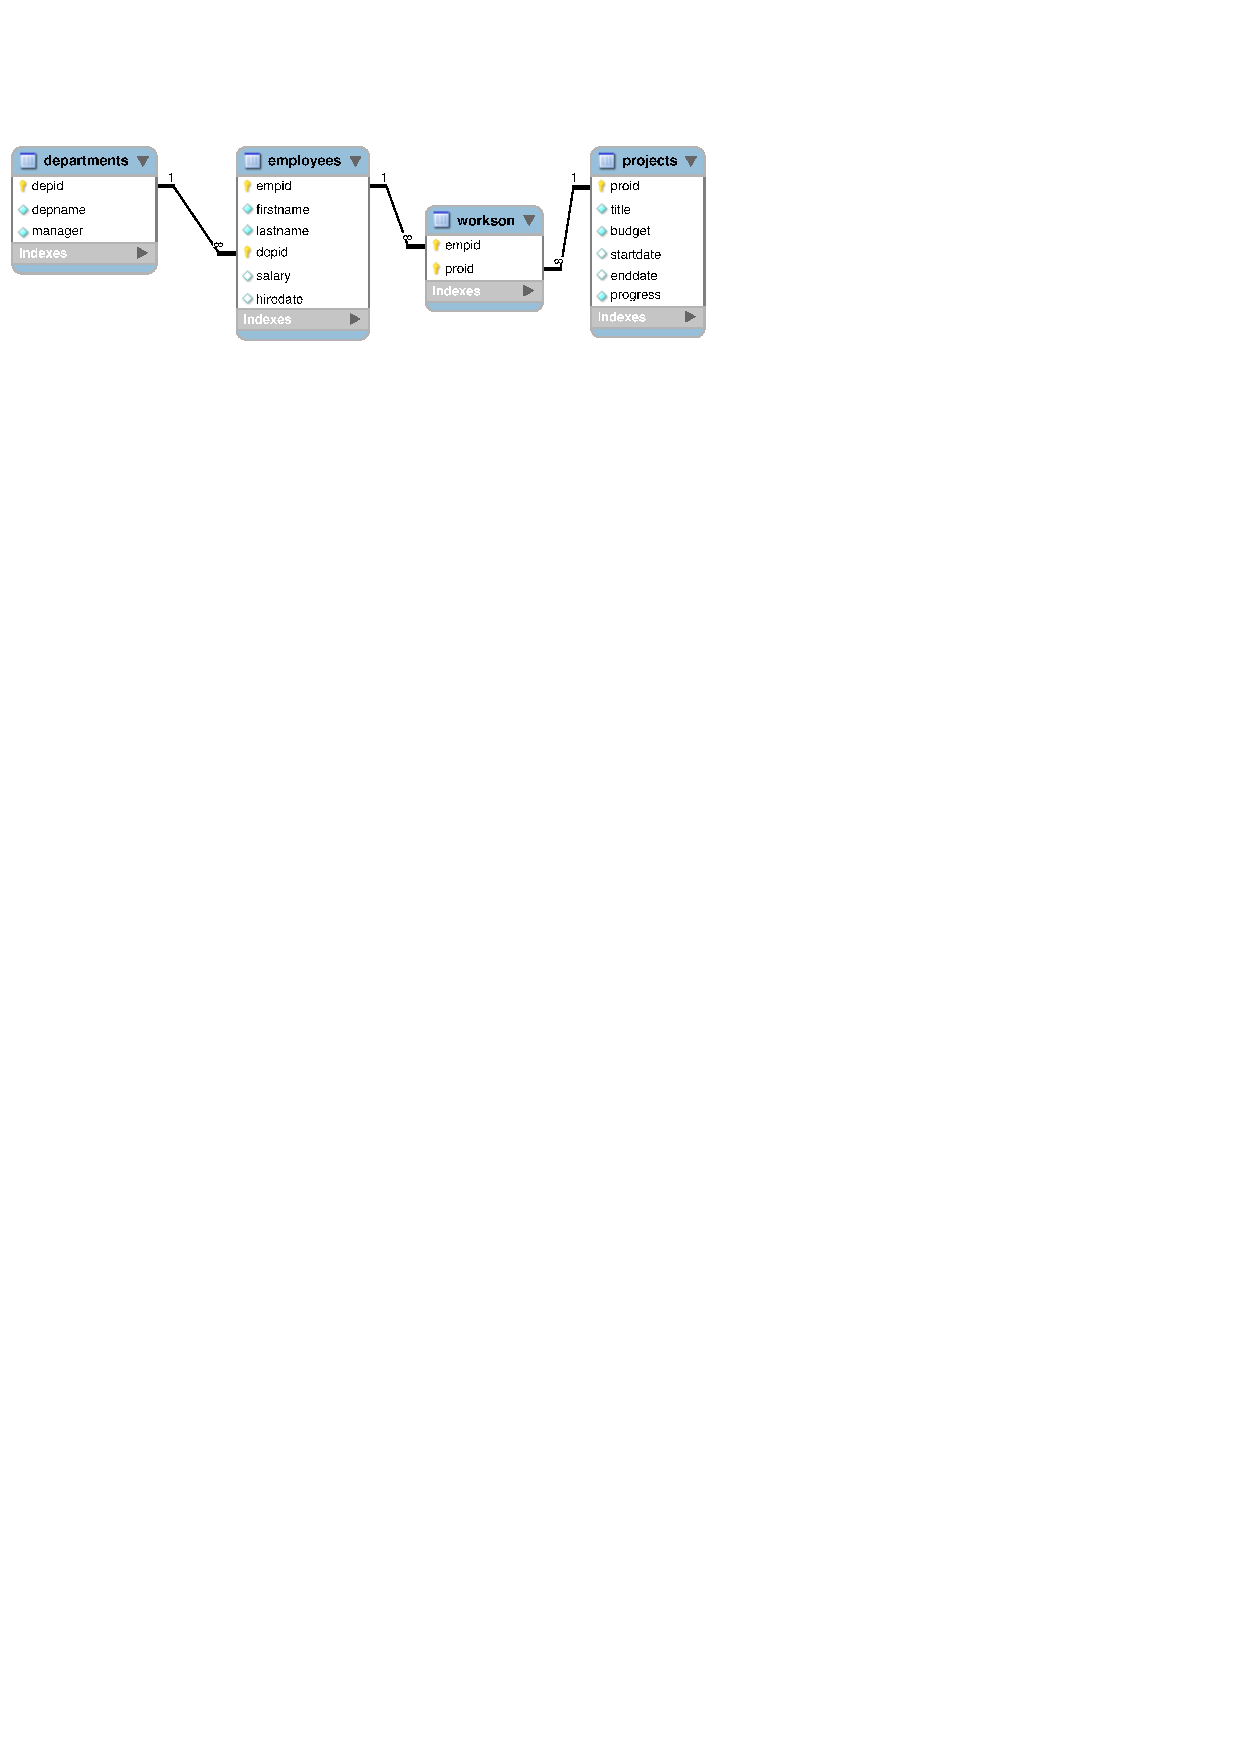
\includegraphics[scale=0.45]{../common/companyREL.pdf} \\
  \bigskip
  \par Το παράδειγμα μιας μικρής σχεσιακής βάσης δεδομένων \\ 
       για τους υπαλλήλους μιας εταιρίας και τα έργα \\
       στα οποία απασχολούνται.
\end{minipage}        
\end{frame}



\begin{frame}
\frametitle{Σχόλια και ερωτήσεις}
\par {\Large \color{red} Σας ευχαριστώ για την προσοχή σας }
\vspace{1cm}
\par Είμαι στη διάθεσή σας για σχόλια, απορίες και ερωτήσεις

\end{frame}


\end{document}